
% Default to the notebook output style

    


% Inherit from the specified cell style.




    
\documentclass[11pt]{article}

    
    
    \usepackage[T1]{fontenc}
    % Nicer default font (+ math font) than Computer Modern for most use cases
    \usepackage{mathpazo}

    % Basic figure setup, for now with no caption control since it's done
    % automatically by Pandoc (which extracts ![](path) syntax from Markdown).
    \usepackage{graphicx}
    % We will generate all images so they have a width \maxwidth. This means
    % that they will get their normal width if they fit onto the page, but
    % are scaled down if they would overflow the margins.
    \makeatletter
    \def\maxwidth{\ifdim\Gin@nat@width>\linewidth\linewidth
    \else\Gin@nat@width\fi}
    \makeatother
    \let\Oldincludegraphics\includegraphics
    % Set max figure width to be 80% of text width, for now hardcoded.
    \renewcommand{\includegraphics}[1]{\Oldincludegraphics[width=.8\maxwidth]{#1}}
    % Ensure that by default, figures have no caption (until we provide a
    % proper Figure object with a Caption API and a way to capture that
    % in the conversion process - todo).
    \usepackage{caption}
    \DeclareCaptionLabelFormat{nolabel}{}
    \captionsetup{labelformat=nolabel}

    \usepackage{adjustbox} % Used to constrain images to a maximum size 
    \usepackage{xcolor} % Allow colors to be defined
    \usepackage{enumerate} % Needed for markdown enumerations to work
    \usepackage{geometry} % Used to adjust the document margins
    \usepackage{amsmath} % Equations
    \usepackage{amssymb} % Equations
    \usepackage{textcomp} % defines textquotesingle
    % Hack from http://tex.stackexchange.com/a/47451/13684:
    \AtBeginDocument{%
        \def\PYZsq{\textquotesingle}% Upright quotes in Pygmentized code
    }
    \usepackage{upquote} % Upright quotes for verbatim code
    \usepackage{eurosym} % defines \euro
    \usepackage[mathletters]{ucs} % Extended unicode (utf-8) support
    \usepackage[utf8x]{inputenc} % Allow utf-8 characters in the tex document
    \usepackage{fancyvrb} % verbatim replacement that allows latex
    \usepackage{grffile} % extends the file name processing of package graphics 
                         % to support a larger range 
    % The hyperref package gives us a pdf with properly built
    % internal navigation ('pdf bookmarks' for the table of contents,
    % internal cross-reference links, web links for URLs, etc.)
    \usepackage{hyperref}
    \usepackage{longtable} % longtable support required by pandoc >1.10
    \usepackage{booktabs}  % table support for pandoc > 1.12.2
    \usepackage[inline]{enumitem} % IRkernel/repr support (it uses the enumerate* environment)
    \usepackage[normalem]{ulem} % ulem is needed to support strikethroughs (\sout)
                                % normalem makes italics be italics, not underlines
    \usepackage{mathrsfs}
    

    
    
    % Colors for the hyperref package
    \definecolor{urlcolor}{rgb}{0,.145,.698}
    \definecolor{linkcolor}{rgb}{.71,0.21,0.01}
    \definecolor{citecolor}{rgb}{.12,.54,.11}

    % ANSI colors
    \definecolor{ansi-black}{HTML}{3E424D}
    \definecolor{ansi-black-intense}{HTML}{282C36}
    \definecolor{ansi-red}{HTML}{E75C58}
    \definecolor{ansi-red-intense}{HTML}{B22B31}
    \definecolor{ansi-green}{HTML}{00A250}
    \definecolor{ansi-green-intense}{HTML}{007427}
    \definecolor{ansi-yellow}{HTML}{DDB62B}
    \definecolor{ansi-yellow-intense}{HTML}{B27D12}
    \definecolor{ansi-blue}{HTML}{208FFB}
    \definecolor{ansi-blue-intense}{HTML}{0065CA}
    \definecolor{ansi-magenta}{HTML}{D160C4}
    \definecolor{ansi-magenta-intense}{HTML}{A03196}
    \definecolor{ansi-cyan}{HTML}{60C6C8}
    \definecolor{ansi-cyan-intense}{HTML}{258F8F}
    \definecolor{ansi-white}{HTML}{C5C1B4}
    \definecolor{ansi-white-intense}{HTML}{A1A6B2}
    \definecolor{ansi-default-inverse-fg}{HTML}{FFFFFF}
    \definecolor{ansi-default-inverse-bg}{HTML}{000000}

    % commands and environments needed by pandoc snippets
    % extracted from the output of `pandoc -s`
    \providecommand{\tightlist}{%
      \setlength{\itemsep}{0pt}\setlength{\parskip}{0pt}}
    \DefineVerbatimEnvironment{Highlighting}{Verbatim}{commandchars=\\\{\}}
    % Add ',fontsize=\small' for more characters per line
    \newenvironment{Shaded}{}{}
    \newcommand{\KeywordTok}[1]{\textcolor[rgb]{0.00,0.44,0.13}{\textbf{{#1}}}}
    \newcommand{\DataTypeTok}[1]{\textcolor[rgb]{0.56,0.13,0.00}{{#1}}}
    \newcommand{\DecValTok}[1]{\textcolor[rgb]{0.25,0.63,0.44}{{#1}}}
    \newcommand{\BaseNTok}[1]{\textcolor[rgb]{0.25,0.63,0.44}{{#1}}}
    \newcommand{\FloatTok}[1]{\textcolor[rgb]{0.25,0.63,0.44}{{#1}}}
    \newcommand{\CharTok}[1]{\textcolor[rgb]{0.25,0.44,0.63}{{#1}}}
    \newcommand{\StringTok}[1]{\textcolor[rgb]{0.25,0.44,0.63}{{#1}}}
    \newcommand{\CommentTok}[1]{\textcolor[rgb]{0.38,0.63,0.69}{\textit{{#1}}}}
    \newcommand{\OtherTok}[1]{\textcolor[rgb]{0.00,0.44,0.13}{{#1}}}
    \newcommand{\AlertTok}[1]{\textcolor[rgb]{1.00,0.00,0.00}{\textbf{{#1}}}}
    \newcommand{\FunctionTok}[1]{\textcolor[rgb]{0.02,0.16,0.49}{{#1}}}
    \newcommand{\RegionMarkerTok}[1]{{#1}}
    \newcommand{\ErrorTok}[1]{\textcolor[rgb]{1.00,0.00,0.00}{\textbf{{#1}}}}
    \newcommand{\NormalTok}[1]{{#1}}
    
    % Additional commands for more recent versions of Pandoc
    \newcommand{\ConstantTok}[1]{\textcolor[rgb]{0.53,0.00,0.00}{{#1}}}
    \newcommand{\SpecialCharTok}[1]{\textcolor[rgb]{0.25,0.44,0.63}{{#1}}}
    \newcommand{\VerbatimStringTok}[1]{\textcolor[rgb]{0.25,0.44,0.63}{{#1}}}
    \newcommand{\SpecialStringTok}[1]{\textcolor[rgb]{0.73,0.40,0.53}{{#1}}}
    \newcommand{\ImportTok}[1]{{#1}}
    \newcommand{\DocumentationTok}[1]{\textcolor[rgb]{0.73,0.13,0.13}{\textit{{#1}}}}
    \newcommand{\AnnotationTok}[1]{\textcolor[rgb]{0.38,0.63,0.69}{\textbf{\textit{{#1}}}}}
    \newcommand{\CommentVarTok}[1]{\textcolor[rgb]{0.38,0.63,0.69}{\textbf{\textit{{#1}}}}}
    \newcommand{\VariableTok}[1]{\textcolor[rgb]{0.10,0.09,0.49}{{#1}}}
    \newcommand{\ControlFlowTok}[1]{\textcolor[rgb]{0.00,0.44,0.13}{\textbf{{#1}}}}
    \newcommand{\OperatorTok}[1]{\textcolor[rgb]{0.40,0.40,0.40}{{#1}}}
    \newcommand{\BuiltInTok}[1]{{#1}}
    \newcommand{\ExtensionTok}[1]{{#1}}
    \newcommand{\PreprocessorTok}[1]{\textcolor[rgb]{0.74,0.48,0.00}{{#1}}}
    \newcommand{\AttributeTok}[1]{\textcolor[rgb]{0.49,0.56,0.16}{{#1}}}
    \newcommand{\InformationTok}[1]{\textcolor[rgb]{0.38,0.63,0.69}{\textbf{\textit{{#1}}}}}
    \newcommand{\WarningTok}[1]{\textcolor[rgb]{0.38,0.63,0.69}{\textbf{\textit{{#1}}}}}
    
    
    % Define a nice break command that doesn't care if a line doesn't already
    % exist.
    \def\br{\hspace*{\fill} \\* }
    % Math Jax compatibility definitions
    \def\gt{>}
    \def\lt{<}
    \let\Oldtex\TeX
    \let\Oldlatex\LaTeX
    \renewcommand{\TeX}{\textrm{\Oldtex}}
    \renewcommand{\LaTeX}{\textrm{\Oldlatex}}
    % Document parameters
    % Document title
    \title{Assignment 1 ME5102}
    
    \author{Aakash \\ Email: \href{mailto:me16b001@iittp.ac.in}{me16b001@iittp.ac.in} \\ Find the code: \href{https://drive.google.com/open?id=1D1zNA7em90M0C5I0VxXinQPLjyuoyLw1}{ Python Code} }
    
    
    

    % Pygments definitions
    
\makeatletter
\def\PY@reset{\let\PY@it=\relax \let\PY@bf=\relax%
    \let\PY@ul=\relax \let\PY@tc=\relax%
    \let\PY@bc=\relax \let\PY@ff=\relax}
\def\PY@tok#1{\csname PY@tok@#1\endcsname}
\def\PY@toks#1+{\ifx\relax#1\empty\else%
    \PY@tok{#1}\expandafter\PY@toks\fi}
\def\PY@do#1{\PY@bc{\PY@tc{\PY@ul{%
    \PY@it{\PY@bf{\PY@ff{#1}}}}}}}
\def\PY#1#2{\PY@reset\PY@toks#1+\relax+\PY@do{#2}}

\expandafter\def\csname PY@tok@w\endcsname{\def\PY@tc##1{\textcolor[rgb]{0.73,0.73,0.73}{##1}}}
\expandafter\def\csname PY@tok@c\endcsname{\let\PY@it=\textit\def\PY@tc##1{\textcolor[rgb]{0.25,0.50,0.50}{##1}}}
\expandafter\def\csname PY@tok@cp\endcsname{\def\PY@tc##1{\textcolor[rgb]{0.74,0.48,0.00}{##1}}}
\expandafter\def\csname PY@tok@k\endcsname{\let\PY@bf=\textbf\def\PY@tc##1{\textcolor[rgb]{0.00,0.50,0.00}{##1}}}
\expandafter\def\csname PY@tok@kp\endcsname{\def\PY@tc##1{\textcolor[rgb]{0.00,0.50,0.00}{##1}}}
\expandafter\def\csname PY@tok@kt\endcsname{\def\PY@tc##1{\textcolor[rgb]{0.69,0.00,0.25}{##1}}}
\expandafter\def\csname PY@tok@o\endcsname{\def\PY@tc##1{\textcolor[rgb]{0.40,0.40,0.40}{##1}}}
\expandafter\def\csname PY@tok@ow\endcsname{\let\PY@bf=\textbf\def\PY@tc##1{\textcolor[rgb]{0.67,0.13,1.00}{##1}}}
\expandafter\def\csname PY@tok@nb\endcsname{\def\PY@tc##1{\textcolor[rgb]{0.00,0.50,0.00}{##1}}}
\expandafter\def\csname PY@tok@nf\endcsname{\def\PY@tc##1{\textcolor[rgb]{0.00,0.00,1.00}{##1}}}
\expandafter\def\csname PY@tok@nc\endcsname{\let\PY@bf=\textbf\def\PY@tc##1{\textcolor[rgb]{0.00,0.00,1.00}{##1}}}
\expandafter\def\csname PY@tok@nn\endcsname{\let\PY@bf=\textbf\def\PY@tc##1{\textcolor[rgb]{0.00,0.00,1.00}{##1}}}
\expandafter\def\csname PY@tok@ne\endcsname{\let\PY@bf=\textbf\def\PY@tc##1{\textcolor[rgb]{0.82,0.25,0.23}{##1}}}
\expandafter\def\csname PY@tok@nv\endcsname{\def\PY@tc##1{\textcolor[rgb]{0.10,0.09,0.49}{##1}}}
\expandafter\def\csname PY@tok@no\endcsname{\def\PY@tc##1{\textcolor[rgb]{0.53,0.00,0.00}{##1}}}
\expandafter\def\csname PY@tok@nl\endcsname{\def\PY@tc##1{\textcolor[rgb]{0.63,0.63,0.00}{##1}}}
\expandafter\def\csname PY@tok@ni\endcsname{\let\PY@bf=\textbf\def\PY@tc##1{\textcolor[rgb]{0.60,0.60,0.60}{##1}}}
\expandafter\def\csname PY@tok@na\endcsname{\def\PY@tc##1{\textcolor[rgb]{0.49,0.56,0.16}{##1}}}
\expandafter\def\csname PY@tok@nt\endcsname{\let\PY@bf=\textbf\def\PY@tc##1{\textcolor[rgb]{0.00,0.50,0.00}{##1}}}
\expandafter\def\csname PY@tok@nd\endcsname{\def\PY@tc##1{\textcolor[rgb]{0.67,0.13,1.00}{##1}}}
\expandafter\def\csname PY@tok@s\endcsname{\def\PY@tc##1{\textcolor[rgb]{0.73,0.13,0.13}{##1}}}
\expandafter\def\csname PY@tok@sd\endcsname{\let\PY@it=\textit\def\PY@tc##1{\textcolor[rgb]{0.73,0.13,0.13}{##1}}}
\expandafter\def\csname PY@tok@si\endcsname{\let\PY@bf=\textbf\def\PY@tc##1{\textcolor[rgb]{0.73,0.40,0.53}{##1}}}
\expandafter\def\csname PY@tok@se\endcsname{\let\PY@bf=\textbf\def\PY@tc##1{\textcolor[rgb]{0.73,0.40,0.13}{##1}}}
\expandafter\def\csname PY@tok@sr\endcsname{\def\PY@tc##1{\textcolor[rgb]{0.73,0.40,0.53}{##1}}}
\expandafter\def\csname PY@tok@ss\endcsname{\def\PY@tc##1{\textcolor[rgb]{0.10,0.09,0.49}{##1}}}
\expandafter\def\csname PY@tok@sx\endcsname{\def\PY@tc##1{\textcolor[rgb]{0.00,0.50,0.00}{##1}}}
\expandafter\def\csname PY@tok@m\endcsname{\def\PY@tc##1{\textcolor[rgb]{0.40,0.40,0.40}{##1}}}
\expandafter\def\csname PY@tok@gh\endcsname{\let\PY@bf=\textbf\def\PY@tc##1{\textcolor[rgb]{0.00,0.00,0.50}{##1}}}
\expandafter\def\csname PY@tok@gu\endcsname{\let\PY@bf=\textbf\def\PY@tc##1{\textcolor[rgb]{0.50,0.00,0.50}{##1}}}
\expandafter\def\csname PY@tok@gd\endcsname{\def\PY@tc##1{\textcolor[rgb]{0.63,0.00,0.00}{##1}}}
\expandafter\def\csname PY@tok@gi\endcsname{\def\PY@tc##1{\textcolor[rgb]{0.00,0.63,0.00}{##1}}}
\expandafter\def\csname PY@tok@gr\endcsname{\def\PY@tc##1{\textcolor[rgb]{1.00,0.00,0.00}{##1}}}
\expandafter\def\csname PY@tok@ge\endcsname{\let\PY@it=\textit}
\expandafter\def\csname PY@tok@gs\endcsname{\let\PY@bf=\textbf}
\expandafter\def\csname PY@tok@gp\endcsname{\let\PY@bf=\textbf\def\PY@tc##1{\textcolor[rgb]{0.00,0.00,0.50}{##1}}}
\expandafter\def\csname PY@tok@go\endcsname{\def\PY@tc##1{\textcolor[rgb]{0.53,0.53,0.53}{##1}}}
\expandafter\def\csname PY@tok@gt\endcsname{\def\PY@tc##1{\textcolor[rgb]{0.00,0.27,0.87}{##1}}}
\expandafter\def\csname PY@tok@err\endcsname{\def\PY@bc##1{\setlength{\fboxsep}{0pt}\fcolorbox[rgb]{1.00,0.00,0.00}{1,1,1}{\strut ##1}}}
\expandafter\def\csname PY@tok@kc\endcsname{\let\PY@bf=\textbf\def\PY@tc##1{\textcolor[rgb]{0.00,0.50,0.00}{##1}}}
\expandafter\def\csname PY@tok@kd\endcsname{\let\PY@bf=\textbf\def\PY@tc##1{\textcolor[rgb]{0.00,0.50,0.00}{##1}}}
\expandafter\def\csname PY@tok@kn\endcsname{\let\PY@bf=\textbf\def\PY@tc##1{\textcolor[rgb]{0.00,0.50,0.00}{##1}}}
\expandafter\def\csname PY@tok@kr\endcsname{\let\PY@bf=\textbf\def\PY@tc##1{\textcolor[rgb]{0.00,0.50,0.00}{##1}}}
\expandafter\def\csname PY@tok@bp\endcsname{\def\PY@tc##1{\textcolor[rgb]{0.00,0.50,0.00}{##1}}}
\expandafter\def\csname PY@tok@fm\endcsname{\def\PY@tc##1{\textcolor[rgb]{0.00,0.00,1.00}{##1}}}
\expandafter\def\csname PY@tok@vc\endcsname{\def\PY@tc##1{\textcolor[rgb]{0.10,0.09,0.49}{##1}}}
\expandafter\def\csname PY@tok@vg\endcsname{\def\PY@tc##1{\textcolor[rgb]{0.10,0.09,0.49}{##1}}}
\expandafter\def\csname PY@tok@vi\endcsname{\def\PY@tc##1{\textcolor[rgb]{0.10,0.09,0.49}{##1}}}
\expandafter\def\csname PY@tok@vm\endcsname{\def\PY@tc##1{\textcolor[rgb]{0.10,0.09,0.49}{##1}}}
\expandafter\def\csname PY@tok@sa\endcsname{\def\PY@tc##1{\textcolor[rgb]{0.73,0.13,0.13}{##1}}}
\expandafter\def\csname PY@tok@sb\endcsname{\def\PY@tc##1{\textcolor[rgb]{0.73,0.13,0.13}{##1}}}
\expandafter\def\csname PY@tok@sc\endcsname{\def\PY@tc##1{\textcolor[rgb]{0.73,0.13,0.13}{##1}}}
\expandafter\def\csname PY@tok@dl\endcsname{\def\PY@tc##1{\textcolor[rgb]{0.73,0.13,0.13}{##1}}}
\expandafter\def\csname PY@tok@s2\endcsname{\def\PY@tc##1{\textcolor[rgb]{0.73,0.13,0.13}{##1}}}
\expandafter\def\csname PY@tok@sh\endcsname{\def\PY@tc##1{\textcolor[rgb]{0.73,0.13,0.13}{##1}}}
\expandafter\def\csname PY@tok@s1\endcsname{\def\PY@tc##1{\textcolor[rgb]{0.73,0.13,0.13}{##1}}}
\expandafter\def\csname PY@tok@mb\endcsname{\def\PY@tc##1{\textcolor[rgb]{0.40,0.40,0.40}{##1}}}
\expandafter\def\csname PY@tok@mf\endcsname{\def\PY@tc##1{\textcolor[rgb]{0.40,0.40,0.40}{##1}}}
\expandafter\def\csname PY@tok@mh\endcsname{\def\PY@tc##1{\textcolor[rgb]{0.40,0.40,0.40}{##1}}}
\expandafter\def\csname PY@tok@mi\endcsname{\def\PY@tc##1{\textcolor[rgb]{0.40,0.40,0.40}{##1}}}
\expandafter\def\csname PY@tok@il\endcsname{\def\PY@tc##1{\textcolor[rgb]{0.40,0.40,0.40}{##1}}}
\expandafter\def\csname PY@tok@mo\endcsname{\def\PY@tc##1{\textcolor[rgb]{0.40,0.40,0.40}{##1}}}
\expandafter\def\csname PY@tok@ch\endcsname{\let\PY@it=\textit\def\PY@tc##1{\textcolor[rgb]{0.25,0.50,0.50}{##1}}}
\expandafter\def\csname PY@tok@cm\endcsname{\let\PY@it=\textit\def\PY@tc##1{\textcolor[rgb]{0.25,0.50,0.50}{##1}}}
\expandafter\def\csname PY@tok@cpf\endcsname{\let\PY@it=\textit\def\PY@tc##1{\textcolor[rgb]{0.25,0.50,0.50}{##1}}}
\expandafter\def\csname PY@tok@c1\endcsname{\let\PY@it=\textit\def\PY@tc##1{\textcolor[rgb]{0.25,0.50,0.50}{##1}}}
\expandafter\def\csname PY@tok@cs\endcsname{\let\PY@it=\textit\def\PY@tc##1{\textcolor[rgb]{0.25,0.50,0.50}{##1}}}

\def\PYZbs{\char`\\}
\def\PYZus{\char`\_}
\def\PYZob{\char`\{}
\def\PYZcb{\char`\}}
\def\PYZca{\char`\^}
\def\PYZam{\char`\&}
\def\PYZlt{\char`\<}
\def\PYZgt{\char`\>}
\def\PYZsh{\char`\#}
\def\PYZpc{\char`\%}
\def\PYZdl{\char`\$}
\def\PYZhy{\char`\-}
\def\PYZsq{\char`\'}
\def\PYZdq{\char`\"}
\def\PYZti{\char`\~}
% for compatibility with earlier versions
\def\PYZat{@}
\def\PYZlb{[}
\def\PYZrb{]}
\makeatother


    % Exact colors from NB
    \definecolor{incolor}{rgb}{0.0, 0.0, 0.5}
    \definecolor{outcolor}{rgb}{0.545, 0.0, 0.0}



    
    % Prevent overflowing lines due to hard-to-break entities
    \sloppy 
    % Setup hyperref package
    \hypersetup{
      breaklinks=true,  % so long urls are correctly broken across lines
      colorlinks=true,
      urlcolor=urlcolor,
      linkcolor=linkcolor,
      citecolor=citecolor,
      }
    % Slightly bigger margins than the latex defaults
    
    \geometry{verbose,tmargin=1in,bmargin=1in,lmargin=1in,rmargin=1in}
    
    

    \begin{document}
    
    
    \maketitle
    
    

    
    \begin{center}\rule{0.5\linewidth}{\linethickness}\end{center}

\section*{Method of weighted
residuals}\label{method-of-weighted-residuals}

Given the differential equation
\[ \frac{d}{dt}\left[x\frac{du}{dx}\right] = \frac{2}{x^2}\] Boundary
conditions \[u(1)=2\] and \[-x\frac{du}{dx}\Biggr|_{x=2} = \frac{1}{2}\]
Assuming the trial function as
\[ u_{h}(x)=a_{0}+a_{1}x+a_{2}x^{2}+\dots +a_{n}x^{n} \] Considering the
first four terms only
\[ u^\sim_{h}(x)=a_{0}+a_{1}x+a_{2}x^{2}+a_{3}x^{3} \] Using boundary
condition 1, we have \[a_{0}+a_{1}+a_{2}+a_{3}=2\] Using boundary
condition 2, we have \[a_{1}+4a_{2}+12a_{3} = -\frac{1}{4}\]
Substituting the above to results in the trial function
\[u^\sim_{h}(x)=2 - \frac{1}{4}(x-1)+a_{2}(x-1)(x-3)+a_{3}(x-1)(x^2+x-11)\]
In order to get the residual, R we substitute our trial function in the
given differential equation
\[ R = \frac{d}{dt}\left[x\frac{du}{dx}\right] - \frac{2}{x^2}\]
\[ \frac{du}{dx} = \dfrac{12 a_3 x^2+8a_2x-48a_3-16a_2-1}{4}\]
\[ R = \dfrac{36 a_3x^2+16a_2x-48a_3-16a_2-1}{4} - \frac{2}{x^2}\]

\subsection*{Exact Solution}\label{exact-solution}

We obtain the following by integrating twice the given differential
equation \[ u(x) = \frac{2}{x}+c_1lnx+c_2\] Finding values of the
integration constants and putting them back
\[ u = \frac{2}{x}+\frac{lnx}{2}\]

    \begin{Verbatim}[commandchars=\\\{\}]
{\color{incolor}In [{\color{incolor}31}]:} \PY{k+kn}{import} \PY{n+nn}{matplotlib}\PY{n+nn}{.}\PY{n+nn}{pyplot} \PY{k}{as} \PY{n+nn}{plt}
         \PY{k+kn}{import} \PY{n+nn}{numpy} \PY{k}{as} \PY{n+nn}{np} 
         
         \PY{n}{x} \PY{o}{=} \PY{n}{np}\PY{o}{.}\PY{n}{arange}\PY{p}{(}\PY{l+m+mi}{1}\PY{p}{,} \PY{l+m+mi}{2}\PY{p}{,} \PY{l+m+mf}{0.01}\PY{p}{)}
         \PY{c+c1}{\PYZsh{}  expression for exact solution}
         \PY{n}{u\PYZus{}exact} \PY{o}{=} \PY{p}{(}\PY{l+m+mi}{2}\PY{o}{/}\PY{n}{x}\PY{p}{)}\PY{o}{+}\PY{l+m+mf}{0.5}\PY{o}{*}\PY{n}{np}\PY{o}{.}\PY{n}{log}\PY{p}{(}\PY{n}{x}\PY{p}{)}
         
         \PY{n}{plt}\PY{o}{.}\PY{n}{plot}\PY{p}{(}\PY{n}{x}\PY{p}{,} \PY{n}{u\PYZus{}exact}\PY{p}{)}
         \PY{n}{plt}\PY{o}{.}\PY{n}{xlabel}\PY{p}{(}\PY{l+s+s1}{\PYZsq{}}\PY{l+s+s1}{x}\PY{l+s+s1}{\PYZsq{}}\PY{p}{,} \PY{n}{fontsize}\PY{o}{=}\PY{l+m+mi}{16}\PY{p}{)}
         \PY{n}{plt}\PY{o}{.}\PY{n}{ylabel}\PY{p}{(}\PY{l+s+s1}{\PYZsq{}}\PY{l+s+s1}{Solution,u}\PY{l+s+s1}{\PYZsq{}}\PY{p}{,} \PY{n}{fontsize}\PY{o}{=}\PY{l+m+mi}{16}\PY{p}{)}
         \PY{n}{plt}\PY{o}{.}\PY{n}{suptitle}\PY{p}{(}\PY{l+s+s1}{\PYZsq{}}\PY{l+s+s1}{Exact Solution}\PY{l+s+s1}{\PYZsq{}}\PY{p}{)}
         \PY{n}{plt}\PY{o}{.}\PY{n}{show}\PY{p}{(}\PY{p}{)}
\end{Verbatim}

    \begin{center}
    \adjustimage{max size={0.9\linewidth}{0.9\paperheight}}{output_1_0.png}
    \end{center}
    { \hspace*{\fill} \\}
    
    \subsection*{Collocation Method}\label{collocation-method}

In the collocation method, we force the residual to be zero at
\({\displaystyle n}\) points
\({\displaystyle x_{1},x_{2},\dots ,x_{n}}\) within the domain.That is
\[R(x_1,a)= 0\] \[R(x_2,a)=0\] \[a = [a_1,a_2]\] From the above equation
we will get the value of \(a\), and solution can be obtained by
substituting it back in our trial function. For our problem, the domain
of interest is \({\displaystyle 1\leq x\leq 2}\). Let us pick two points
in this domain \({\displaystyle x_{1}}\) and \({\displaystyle x_{2}}\)
such that \({\displaystyle 1\leq x_{1}<x_{2}\leq 2}\). In this example
we choose \({\displaystyle x_{1}=4/3}\) and
\({\displaystyle x_{2}=5/3}\). \\
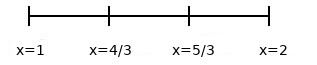
\includegraphics{col}


    \begin{Verbatim}[commandchars=\\\{\}]
{\color{incolor}In [{\color{incolor}33}]:} \PY{k+kn}{import} \PY{n+nn}{matplotlib}\PY{n+nn}{.}\PY{n+nn}{pyplot} \PY{k}{as} \PY{n+nn}{plt}
         \PY{k+kn}{import} \PY{n+nn}{numpy} \PY{k}{as} \PY{n+nn}{np} 
         \PY{k+kn}{from} \PY{n+nn}{sympy} \PY{k}{import} \PY{o}{*}
         
         \PY{n}{a\PYZus{}col} \PY{o}{=} \PY{n}{Symbol}\PY{p}{(}\PY{l+s+s1}{\PYZsq{}}\PY{l+s+s1}{a}\PY{l+s+s1}{\PYZsq{}}\PY{p}{)}
         \PY{n}{b\PYZus{}col} \PY{o}{=} \PY{n}{Symbol}\PY{p}{(}\PY{l+s+s1}{\PYZsq{}}\PY{l+s+s1}{b}\PY{l+s+s1}{\PYZsq{}}\PY{p}{)}
         \PY{n}{val\PYZus{}col} \PY{o}{=} \PY{p}{[}\PY{l+m+mi}{4}\PY{o}{/}\PY{l+m+mi}{3} \PY{p}{,}\PY{l+m+mi}{5}\PY{o}{/}\PY{l+m+mi}{3}\PY{p}{]}
         \PY{n}{eqn\PYZus{}col} \PY{o}{=}\PY{p}{[}\PY{p}{]}
         
         \PY{k}{def} \PY{n+nf}{function}\PY{p}{(}\PY{n}{x}\PY{p}{)}\PY{p}{:}
         	\PY{k}{for} \PY{n}{x} \PY{o+ow}{in} \PY{n}{val\PYZus{}col}\PY{p}{:}
         		\PY{c+c1}{\PYZsh{} calculating residuals }
         		\PY{n}{eqn\PYZus{}col}\PY{o}{.}\PY{n}{append}\PY{p}{(}\PY{o}{\PYZhy{}}\PY{l+m+mf}{0.25}\PY{o}{+}\PY{l+m+mi}{4}\PY{o}{*}\PY{p}{(}\PY{n}{x}\PY{o}{\PYZhy{}}\PY{l+m+mi}{1}\PY{p}{)}\PY{o}{*}\PY{n}{a\PYZus{}col}\PY{o}{+}\PY{l+m+mi}{3}\PY{o}{*}\PY{p}{(}\PY{l+m+mi}{3}\PY{o}{*}\PY{p}{(}\PY{n}{x}\PY{o}{*}\PY{o}{*}\PY{l+m+mi}{2}\PY{p}{)}\PY{o}{\PYZhy{}}\PY{l+m+mi}{4}\PY{p}{)}\PY{o}{*}\PY{n}{b\PYZus{}col}\PY{o}{\PYZhy{}}\PY{p}{(}\PY{l+m+mi}{2}\PY{o}{/}\PY{p}{(}\PY{n}{x}\PY{o}{*}\PY{o}{*}\PY{l+m+mi}{2}\PY{p}{)}\PY{p}{)}\PY{p}{)}
         	\PY{k}{return}\PY{p}{(}\PY{n}{eqn\PYZus{}col}\PY{p}{)}
         
         \PY{n}{solve}\PY{p}{(}\PY{n}{function}\PY{p}{(}\PY{n}{val\PYZus{}col}\PY{p}{)}\PY{p}{,} \PY{p}{[}\PY{n}{a\PYZus{}col}\PY{p}{,}\PY{n}{b\PYZus{}col}\PY{p}{]}\PY{p}{)}
         \PY{n+nb}{print}\PY{p}{(}\PY{l+s+s2}{\PYZdq{}}\PY{l+s+s2}{eqn}\PY{l+s+s2}{\PYZdq{}}\PY{p}{,}\PY{n}{eqn\PYZus{}col}\PY{p}{)}
         
         \PY{n}{z\PYZus{}col} \PY{o}{=} \PY{n}{solve}\PY{p}{(}\PY{n}{function}\PY{p}{(}\PY{n}{val\PYZus{}col}\PY{p}{)}\PY{p}{,} \PY{p}{[}\PY{n}{a\PYZus{}col}\PY{p}{,}\PY{n}{b\PYZus{}col}\PY{p}{]}\PY{p}{)}
         \PY{n+nb}{print}\PY{p}{(}\PY{l+s+s2}{\PYZdq{}}\PY{l+s+s2}{a }\PY{l+s+s2}{\PYZdq{}}\PY{p}{,}\PY{n}{z}\PY{o}{.}\PY{n}{get}\PY{p}{(}\PY{n}{a\PYZus{}col}\PY{p}{)}\PY{p}{)}
         \PY{n+nb}{print}\PY{p}{(}\PY{l+s+s2}{\PYZdq{}}\PY{l+s+s2}{b }\PY{l+s+s2}{\PYZdq{}}\PY{p}{,}\PY{n}{z}\PY{o}{.}\PY{n}{get}\PY{p}{(}\PY{n}{b\PYZus{}col}\PY{p}{)}\PY{p}{)}
         
         \PY{n}{x} \PY{o}{=} \PY{n}{np}\PY{o}{.}\PY{n}{arange}\PY{p}{(}\PY{l+m+mi}{1}\PY{p}{,} \PY{l+m+mi}{2}\PY{p}{,} \PY{l+m+mf}{0.01}\PY{p}{)}
         \PY{n}{u\PYZus{}col} \PY{o}{=} \PY{l+m+mf}{2.} \PY{o}{\PYZhy{}} \PY{p}{(}\PY{l+m+mf}{0.25}\PY{p}{)}\PY{o}{*}\PY{p}{(}\PY{n}{x}\PY{o}{\PYZhy{}}\PY{l+m+mi}{1}\PY{p}{)}\PY{o}{+}\PY{p}{(}\PY{n}{x}\PY{o}{\PYZhy{}}\PY{l+m+mi}{1}\PY{p}{)}\PY{o}{*}\PY{p}{(}\PY{n}{x}\PY{o}{\PYZhy{}}\PY{l+m+mi}{3}\PY{p}{)}\PY{o}{*}\PY{n}{z\PYZus{}col}\PY{o}{.}\PY{n}{get}  \PY{p}{(}\PY{n}{a\PYZus{}col}\PY{p}{)}\PY{o}{+}\PY{p}{(}\PY{n}{x}\PY{o}{\PYZhy{}}\PY{l+m+mi}{1}\PY{p}{)}\PY{o}{*}\PY{p}{(}\PY{n}{x}\PY{o}{*}\PY{o}{*}\PY{l+m+mi}{2}\PY{o}{+}\PY{n}{x}\PY{o}{\PYZhy{}}\PY{l+m+mi}{11}\PY{p}{)}\PY{o}{*}\PY{n}{z\PYZus{}col}\PY{o}{.}\PY{n}{get}\PY{p}{(}\PY{n}{b\PYZus{}col}\PY{p}{)}
         \PY{n}{plt}\PY{o}{.}\PY{n}{plot}\PY{p}{(}\PY{n}{x}\PY{p}{,} \PY{n}{u\PYZus{}col}\PY{p}{)}
         \PY{n}{plt}\PY{o}{.}\PY{n}{xlabel}\PY{p}{(}\PY{l+s+s1}{\PYZsq{}}\PY{l+s+s1}{x}\PY{l+s+s1}{\PYZsq{}}\PY{p}{,} \PY{n}{fontsize}\PY{o}{=}\PY{l+m+mi}{16}\PY{p}{)}
         \PY{n}{plt}\PY{o}{.}\PY{n}{ylabel}\PY{p}{(}\PY{l+s+s1}{\PYZsq{}}\PY{l+s+s1}{Solution,u}\PY{l+s+s1}{\PYZsq{}}\PY{p}{,} \PY{n}{fontsize}\PY{o}{=}\PY{l+m+mi}{16}\PY{p}{)}
         \PY{n}{plt}\PY{o}{.}\PY{n}{suptitle}\PY{p}{(}\PY{l+s+s1}{\PYZsq{}}\PY{l+s+s1}{Solution by Collocation method}\PY{l+s+s1}{\PYZsq{}}\PY{p}{)}
         \PY{n}{plt}\PY{o}{.}\PY{n}{show}\PY{p}{(}\PY{p}{)}
\end{Verbatim}

    \begin{Verbatim}[commandchars=\\\{\}]
eqn [1.33333333333333*a + 4.0*b - 1.375, 2.66666666666667*a + 13.0*b - 0.97]
a  2.09925000000000
b  -0.356000000000000

    \end{Verbatim}

    \begin{center}
    \adjustimage{max size={0.9\linewidth}{0.9\paperheight}}{output_3_1.png}
    \end{center}
    { \hspace*{\fill} \\}
    
    \subsection*{Subdomain Method}\label{subdomain-method}

The subdomain method is another way of forcing the residuals to zero. In
this method, we let the "average" of the residual vanish over each
domain.
\[{\displaystyle {\frac {1}{\Delta x_{i}}}\int _{\Delta x_{i}}R(x)dx=0}\]
\[{\displaystyle {\frac {1}{\Delta x_{1}}}\int _{1}^{\frac {3}{2}}R(x)dx=-\frac{19}{24}+2a_{2}+{\frac {9}{8}}a_{3} = 0 \qquad {\text{and}}~\qquad {\frac {1}{\Delta x_{2}}}\int _{\frac {3}{2}}^{2}R(x)dx=-\frac{11}{24}+{\frac {3}{2}}a_{2}+{\frac {63}{8}}a_{3}} = 0\]
solving the above for \(a\) and substituiting it back in the trial
function.

    \begin{Verbatim}[commandchars=\\\{\}]
{\color{incolor}In [{\color{incolor}34}]:} \PY{k+kn}{from} \PY{n+nn}{sympy} \PY{k}{import} \PY{o}{*}
         \PY{k+kn}{import} \PY{n+nn}{matplotlib}\PY{n+nn}{.}\PY{n+nn}{pyplot} \PY{k}{as} \PY{n+nn}{plt}
         \PY{k+kn}{import} \PY{n+nn}{numpy} \PY{k}{as} \PY{n+nn}{np}
         \PY{k+kn}{import} \PY{n+nn}{matplotlib}\PY{n+nn}{.}\PY{n+nn}{patches} \PY{k}{as} \PY{n+nn}{mpatches}
         
         \PY{n}{a\PYZus{}sub} \PY{o}{=} \PY{n}{Symbol}\PY{p}{(}\PY{l+s+s1}{\PYZsq{}}\PY{l+s+s1}{a}\PY{l+s+s1}{\PYZsq{}}\PY{p}{)}
         \PY{n}{b\PYZus{}sub} \PY{o}{=} \PY{n}{Symbol}\PY{p}{(}\PY{l+s+s1}{\PYZsq{}}\PY{l+s+s1}{b}\PY{l+s+s1}{\PYZsq{}}\PY{p}{)}
         \PY{n}{x\PYZus{}sub} \PY{o}{=} \PY{n}{Symbol}\PY{p}{(}\PY{l+s+s1}{\PYZsq{}}\PY{l+s+s1}{x\PYZus{}sub}\PY{l+s+s1}{\PYZsq{}}\PY{p}{)}
         \PY{n}{eqn\PYZus{}sub} \PY{o}{=}\PY{p}{[}\PY{p}{]}
         \PY{n}{eqn\PYZus{}sub}\PY{o}{.}\PY{n}{append}\PY{p}{(}\PY{n}{integrate}\PY{p}{(}\PY{o}{\PYZhy{}}\PY{l+m+mf}{0.25}\PY{o}{+}\PY{l+m+mi}{4}\PY{o}{*}\PY{p}{(}\PY{o}{\PYZhy{}}\PY{l+m+mi}{1}\PY{p}{)}\PY{o}{*}\PY{n}{a\PYZus{}sub}\PY{o}{+}\PY{l+m+mi}{3}\PY{o}{*}\PY{p}{(}\PY{l+m+mi}{3}\PY{o}{*}\PY{p}{(}\PY{n}{x\PYZus{}sub}\PY{o}{*}\PY{o}{*}\PY{l+m+mi}{2}\PY{p}{)}\PY{o}{\PYZhy{}}\PY{l+m+mi}{4}\PY{p}{)}\PY{o}{*}\PY{n}{b\PYZus{}sub}\PY{o}{\PYZhy{}}\PY{p}{(}\PY{l+m+mi}{2}\PY{o}{/}\PY{p}{(}\PY{n}{x\PYZus{}sub}\PY{o}{*}\PY{o}{*}\PY{l+m+mi}{2}\PY{p}{)}\PY{p}{)}\PY{p}{,} \PY{p}{(}\PY{n}{x\PYZus{}sub}\PY{p}{,} \PY{l+m+mi}{1}\PY{p}{,} \PY{l+m+mf}{1.5}\PY{p}{)}\PY{p}{)}\PY{p}{)}
         \PY{n}{eqn\PYZus{}sub}\PY{o}{.}\PY{n}{append}\PY{p}{(}\PY{n}{integrate}\PY{p}{(}\PY{o}{\PYZhy{}}\PY{l+m+mf}{0.25}\PY{o}{+}\PY{l+m+mi}{4}\PY{o}{*}\PY{p}{(}\PY{n}{x\PYZus{}sub}\PY{o}{\PYZhy{}}\PY{l+m+mi}{1}\PY{p}{)}\PY{o}{*}\PY{n}{a\PYZus{}sub}\PY{o}{+}\PY{l+m+mi}{3}\PY{o}{*}\PY{p}{(}\PY{l+m+mi}{3}\PY{o}{*}\PY{p}{(}\PY{n}{x\PYZus{}sub}\PY{o}{*}\PY{o}{*}\PY{l+m+mi}{2}\PY{p}{)}\PY{o}{\PYZhy{}}\PY{l+m+mi}{4}\PY{p}{)}\PY{o}{*}\PY{n}{b\PYZus{}sub}\PY{o}{\PYZhy{}}\PY{p}{(}\PY{l+m+mi}{2}\PY{o}{/}\PY{p}{(}\PY{n}{x\PYZus{}sub}\PY{o}{*}\PY{o}{*}\PY{l+m+mi}{2}\PY{p}{)}\PY{p}{)}\PY{p}{,} \PY{p}{(}\PY{n}{x\PYZus{}sub}\PY{p}{,} \PY{l+m+mf}{1.5}\PY{p}{,} \PY{l+m+mi}{2}\PY{p}{)}\PY{p}{)}\PY{p}{)}
         \PY{n}{z\PYZus{}sub} \PY{o}{=} \PY{n}{solve}\PY{p}{(}\PY{n}{eqn\PYZus{}sub}\PY{p}{,} \PY{p}{[}\PY{n}{a\PYZus{}sub}\PY{p}{,}\PY{n}{b\PYZus{}sub}\PY{p}{]}\PY{p}{)}
         \PY{n+nb}{print}\PY{p}{(}\PY{l+s+s2}{\PYZdq{}}\PY{l+s+s2}{a}\PY{l+s+s2}{\PYZdq{}}\PY{p}{,}\PY{n}{z\PYZus{}sub}\PY{o}{.}\PY{n}{get}\PY{p}{(}\PY{n}{a\PYZus{}sub}\PY{p}{)}\PY{p}{)}
         \PY{n+nb}{print}\PY{p}{(}\PY{l+s+s2}{\PYZdq{}}\PY{l+s+s2}{b}\PY{l+s+s2}{\PYZdq{}}\PY{p}{,}\PY{n}{z\PYZus{}sub}\PY{o}{.}\PY{n}{get}\PY{p}{(}\PY{n}{b\PYZus{}sub}\PY{p}{)}\PY{p}{)}
         \PY{n}{x\PYZus{}sub} \PY{o}{=} \PY{n}{np}\PY{o}{.}\PY{n}{arange}\PY{p}{(}\PY{l+m+mi}{1}\PY{p}{,} \PY{l+m+mf}{2.}\PY{p}{,} \PY{l+m+mf}{0.01}\PY{p}{)}
         \PY{n}{u\PYZus{}sub} \PY{o}{=} \PY{l+m+mi}{2} \PY{o}{\PYZhy{}} \PY{l+m+mf}{0.25}\PY{o}{*}\PY{p}{(}\PY{n}{x\PYZus{}sub}\PY{o}{\PYZhy{}}\PY{l+m+mi}{1}\PY{p}{)}\PY{o}{+}\PY{p}{(}\PY{n}{x\PYZus{}sub}\PY{o}{\PYZhy{}}\PY{l+m+mi}{1}\PY{p}{)}\PY{o}{*}\PY{p}{(}\PY{n}{x\PYZus{}sub}\PY{o}{\PYZhy{}}\PY{l+m+mi}{3}\PY{p}{)}\PY{o}{*}\PY{n}{z\PYZus{}sub}\PY{o}{.}\PY{n}{get}\PY{p}{(}\PY{n}{a\PYZus{}sub}\PY{p}{)}\PY{o}{+}\PY{p}{(}\PY{n}{x\PYZus{}sub}\PY{o}{\PYZhy{}}\PY{l+m+mi}{1}\PY{p}{)}\PY{o}{*}\PY{p}{(}\PY{n}{x\PYZus{}sub}\PY{o}{*}\PY{o}{*}\PY{l+m+mi}{2}\PY{o}{+}\PY{n}{x\PYZus{}sub}\PY{o}{\PYZhy{}}\PY{l+m+mi}{11}\PY{p}{)}\PY{o}{*}\PY{n}{z\PYZus{}sub}\PY{o}{.}\PY{n}{get}\PY{p}{(}\PY{n}{b\PYZus{}sub}\PY{p}{)}
         
         \PY{n}{plt}\PY{o}{.}\PY{n}{plot}\PY{p}{(}\PY{n}{x\PYZus{}sub}\PY{p}{,} \PY{n}{u\PYZus{}sub} \PY{p}{,} \PY{n}{color}\PY{o}{=}\PY{l+s+s1}{\PYZsq{}}\PY{l+s+s1}{b}\PY{l+s+s1}{\PYZsq{}}\PY{p}{,} \PY{n}{label}\PY{o}{=}\PY{l+s+s2}{\PYZdq{}}\PY{l+s+s2}{Subdomain}\PY{l+s+s2}{\PYZdq{}}\PY{p}{)}
         \PY{n}{plt}\PY{o}{.}\PY{n}{xlabel}\PY{p}{(}\PY{l+s+s1}{\PYZsq{}}\PY{l+s+s1}{x}\PY{l+s+s1}{\PYZsq{}}\PY{p}{,} \PY{n}{fontsize}\PY{o}{=}\PY{l+m+mi}{16}\PY{p}{)}
         \PY{n}{plt}\PY{o}{.}\PY{n}{ylabel}\PY{p}{(}\PY{l+s+s1}{\PYZsq{}}\PY{l+s+s1}{Solution,u}\PY{l+s+s1}{\PYZsq{}}\PY{p}{,} \PY{n}{fontsize}\PY{o}{=}\PY{l+m+mi}{16}\PY{p}{)}
         \PY{n}{plt}\PY{o}{.}\PY{n}{suptitle}\PY{p}{(}\PY{l+s+s1}{\PYZsq{}}\PY{l+s+s1}{Solution by Subdomain method}\PY{l+s+s1}{\PYZsq{}}\PY{p}{)}
         \PY{n}{plt}\PY{o}{.}\PY{n}{show}\PY{p}{(}\PY{p}{)}
\end{Verbatim}

    \begin{Verbatim}[commandchars=\\\{\}]
a -0.327956989247312
b 0.120669056152927

    \end{Verbatim}

    \begin{center}
    \adjustimage{max size={0.9\linewidth}{0.9\paperheight}}{output_5_1.png}
    \end{center}
    { \hspace*{\fill} \\}
    
    \subsection*{Galerkin Method}\label{galerkin-method}

    \begin{Verbatim}[commandchars=\\\{\}]
{\color{incolor}In [{\color{incolor}36}]:} \PY{k+kn}{from} \PY{n+nn}{sympy} \PY{k}{import} \PY{o}{*}
         \PY{k+kn}{import} \PY{n+nn}{matplotlib}\PY{n+nn}{.}\PY{n+nn}{pyplot} \PY{k}{as} \PY{n+nn}{plt}
         \PY{k+kn}{import} \PY{n+nn}{numpy} \PY{k}{as} \PY{n+nn}{np} 
         \PY{k+kn}{import} \PY{n+nn}{matplotlib}\PY{n+nn}{.}\PY{n+nn}{patches} \PY{k}{as} \PY{n+nn}{mpatches}
         
         \PY{n}{a\PYZus{}gal} \PY{o}{=} \PY{n}{Symbol}\PY{p}{(}\PY{l+s+s1}{\PYZsq{}}\PY{l+s+s1}{a}\PY{l+s+s1}{\PYZsq{}}\PY{p}{)}
         \PY{n}{b\PYZus{}gal} \PY{o}{=} \PY{n}{Symbol}\PY{p}{(}\PY{l+s+s1}{\PYZsq{}}\PY{l+s+s1}{b}\PY{l+s+s1}{\PYZsq{}}\PY{p}{)}
         \PY{n}{x\PYZus{}gal} \PY{o}{=} \PY{n}{Symbol}\PY{p}{(}\PY{l+s+s1}{\PYZsq{}}\PY{l+s+s1}{x}\PY{l+s+s1}{\PYZsq{}}\PY{p}{)}
         \PY{n}{eqn\PYZus{}gal} \PY{o}{=}\PY{p}{[}\PY{p}{]}
         \PY{n}{r\PYZus{}gal} \PY{o}{=} \PY{o}{\PYZhy{}}\PY{l+m+mf}{0.25}\PY{o}{+}\PY{l+m+mi}{4}\PY{o}{*}\PY{p}{(}\PY{n}{x\PYZus{}gal}\PY{o}{\PYZhy{}}\PY{l+m+mi}{1}\PY{p}{)}\PY{o}{*}\PY{n}{a\PYZus{}gal}\PY{o}{+}\PY{l+m+mi}{3}\PY{o}{*}\PY{p}{(}\PY{l+m+mi}{3}\PY{o}{*}\PY{p}{(}\PY{n}{x\PYZus{}gal}\PY{o}{*}\PY{o}{*}\PY{l+m+mi}{2}\PY{p}{)}\PY{o}{\PYZhy{}}\PY{l+m+mi}{4}\PY{p}{)}\PY{o}{*}\PY{n}{b\PYZus{}gal}\PY{o}{\PYZhy{}}\PY{p}{(}\PY{l+m+mi}{2}\PY{o}{/}\PY{p}{(}\PY{n}{x\PYZus{}gal}\PY{o}{*}\PY{o}{*}\PY{l+m+mi}{2}\PY{p}{)}\PY{p}{)}
         \PY{n+nb}{print}\PY{p}{(}\PY{n}{diff}\PY{p}{(}\PY{n}{r\PYZus{}gal}\PY{p}{,}\PY{n}{a\PYZus{}gal}\PY{p}{)}\PY{p}{)}
         \PY{n}{eqn\PYZus{}gal}\PY{o}{.}\PY{n}{append}\PY{p}{(}\PY{n}{integrate}\PY{p}{(}\PY{n}{r\PYZus{}gal}\PY{o}{*}\PY{n}{x\PYZus{}gal}\PY{p}{,} \PY{p}{(}\PY{n}{x\PYZus{}gal}\PY{p}{,} \PY{l+m+mi}{1}\PY{p}{,} \PY{l+m+mi}{2}\PY{p}{)}\PY{p}{)}\PY{p}{)}
         \PY{n}{eqn\PYZus{}gal}\PY{o}{.}\PY{n}{append}\PY{p}{(}\PY{n}{integrate}\PY{p}{(}\PY{n}{r\PYZus{}gal}\PY{o}{*}\PY{n}{x\PYZus{}gal}\PY{o}{*}\PY{n}{x\PYZus{}gal}\PY{p}{,} \PY{p}{(}\PY{n}{x\PYZus{}gal}\PY{p}{,} \PY{l+m+mi}{1}\PY{p}{,} \PY{l+m+mi}{2}\PY{p}{)}\PY{p}{)}\PY{p}{)}
         \PY{n+nb}{print}\PY{p}{(}\PY{n}{eqn\PYZus{}gal}\PY{p}{)}
         \PY{n}{z\PYZus{}gal} \PY{o}{=} \PY{n}{solve}\PY{p}{(}\PY{n}{eqn\PYZus{}gal}\PY{p}{,} \PY{p}{[}\PY{n}{a\PYZus{}gal}\PY{p}{,}\PY{n}{b\PYZus{}gal}\PY{p}{]}\PY{p}{)}
         
         \PY{n}{x} \PY{o}{=} \PY{n}{np}\PY{o}{.}\PY{n}{arange}\PY{p}{(}\PY{l+m+mi}{1}\PY{p}{,} \PY{l+m+mf}{2.}\PY{p}{,} \PY{l+m+mf}{0.01}\PY{p}{)}
         \PY{n}{u\PYZus{}gal} \PY{o}{=} \PY{l+m+mi}{2} \PY{o}{\PYZhy{}} \PY{l+m+mf}{0.25}\PY{o}{*}\PY{p}{(}\PY{n}{x}\PY{o}{\PYZhy{}}\PY{l+m+mi}{1}\PY{p}{)}\PY{o}{+}\PY{p}{(}\PY{n}{x}\PY{o}{\PYZhy{}}\PY{l+m+mi}{1}\PY{p}{)}\PY{o}{*}\PY{p}{(}\PY{n}{x}\PY{o}{\PYZhy{}}\PY{l+m+mi}{3}\PY{p}{)}\PY{o}{*}\PY{n}{z\PYZus{}gal}\PY{o}{.}\PY{n}{get}\PY{p}{(}\PY{n}{a\PYZus{}gal}\PY{p}{)}\PY{o}{+}\PY{p}{(}\PY{n}{x}\PY{o}{\PYZhy{}}\PY{l+m+mi}{1}\PY{p}{)}\PY{o}{*}\PY{p}{(}\PY{p}{(}\PY{n}{x}\PY{o}{*}\PY{o}{*}\PY{l+m+mi}{2}\PY{p}{)}\PY{o}{+}\PY{n}{x}\PY{o}{\PYZhy{}}\PY{l+m+mi}{11}\PY{p}{)}\PY{o}{*}\PY{n}{z\PYZus{}gal}\PY{o}{.}\PY{n}{get}\PY{p}{(}\PY{n}{b\PYZus{}gal}\PY{p}{)}
         \PY{n}{plt}\PY{o}{.}\PY{n}{plot}\PY{p}{(}\PY{n}{x}\PY{p}{,} \PY{n}{u\PYZus{}gal} \PY{p}{,} \PY{n}{color}\PY{o}{=}\PY{l+s+s1}{\PYZsq{}}\PY{l+s+s1}{b}\PY{l+s+s1}{\PYZsq{}}\PY{p}{)}
         \PY{n}{plt}\PY{o}{.}\PY{n}{xlabel}\PY{p}{(}\PY{l+s+s1}{\PYZsq{}}\PY{l+s+s1}{x}\PY{l+s+s1}{\PYZsq{}}\PY{p}{,} \PY{n}{fontsize}\PY{o}{=}\PY{l+m+mi}{16}\PY{p}{)}
         \PY{n}{plt}\PY{o}{.}\PY{n}{ylabel}\PY{p}{(}\PY{l+s+s1}{\PYZsq{}}\PY{l+s+s1}{Solution,u}\PY{l+s+s1}{\PYZsq{}}\PY{p}{,} \PY{n}{fontsize}\PY{o}{=}\PY{l+m+mi}{16}\PY{p}{)}
         \PY{n}{plt}\PY{o}{.}\PY{n}{suptitle}\PY{p}{(}\PY{l+s+s1}{\PYZsq{}}\PY{l+s+s1}{Solution by Galerkin method}\PY{l+s+s1}{\PYZsq{}}\PY{p}{)}
         
         \PY{n}{plt}\PY{o}{.}\PY{n}{show}\PY{p}{(}\PY{p}{)}
\end{Verbatim}

    \begin{Verbatim}[commandchars=\\\{\}]
4*x - 4
[3.33333333333333*a + 15.75*b - 2.0*log(2) - 0.375, 5.66666666666667*a + 27.8*b - 2.58333333333333]

    \end{Verbatim}

    \begin{center}
    \adjustimage{max size={0.9\linewidth}{0.9\paperheight}}{output_7_1.png}
    \end{center}
    { \hspace*{\fill} \\}
    
    \subsection*{Least Squares Method}\label{least-squares-method}

In this method we force the residuals to be zero as
\[{\int _{0}^{1}R(x)~{\frac {\partial R(x)}{\partial a_{i}}}~dx=0}\]

    \begin{Verbatim}[commandchars=\\\{\}]
{\color{incolor}In [{\color{incolor}37}]:} \PY{k+kn}{from} \PY{n+nn}{sympy} \PY{k}{import} \PY{o}{*}
         \PY{k+kn}{import} \PY{n+nn}{matplotlib}\PY{n+nn}{.}\PY{n+nn}{pyplot} \PY{k}{as} \PY{n+nn}{plt}
         \PY{k+kn}{import} \PY{n+nn}{numpy} \PY{k}{as} \PY{n+nn}{np} 
         \PY{k+kn}{import} \PY{n+nn}{matplotlib}\PY{n+nn}{.}\PY{n+nn}{patches} \PY{k}{as} \PY{n+nn}{mpatches}
         
         \PY{n}{a\PYZus{}lea} \PY{o}{=} \PY{n}{Symbol}\PY{p}{(}\PY{l+s+s1}{\PYZsq{}}\PY{l+s+s1}{a}\PY{l+s+s1}{\PYZsq{}}\PY{p}{)}
         \PY{n}{b\PYZus{}lea} \PY{o}{=} \PY{n}{Symbol}\PY{p}{(}\PY{l+s+s1}{\PYZsq{}}\PY{l+s+s1}{b}\PY{l+s+s1}{\PYZsq{}}\PY{p}{)}
         \PY{n}{x\PYZus{}lea} \PY{o}{=} \PY{n}{Symbol}\PY{p}{(}\PY{l+s+s1}{\PYZsq{}}\PY{l+s+s1}{x}\PY{l+s+s1}{\PYZsq{}}\PY{p}{)}
         \PY{n}{eqn\PYZus{}lea} \PY{o}{=}\PY{p}{[}\PY{p}{]}
         \PY{n}{r\PYZus{}lea} \PY{o}{=} \PY{o}{\PYZhy{}}\PY{l+m+mf}{0.25}\PY{o}{+}\PY{l+m+mi}{4}\PY{o}{*}\PY{p}{(}\PY{n}{x\PYZus{}lea}\PY{o}{\PYZhy{}}\PY{l+m+mi}{1}\PY{p}{)}\PY{o}{*}\PY{n}{a\PYZus{}lea}\PY{o}{+}\PY{l+m+mi}{3}\PY{o}{*}\PY{p}{(}\PY{l+m+mi}{3}\PY{o}{*}\PY{p}{(}\PY{n}{x\PYZus{}lea}\PY{o}{*}\PY{o}{*}\PY{l+m+mi}{2}\PY{p}{)}\PY{o}{\PYZhy{}}\PY{l+m+mi}{4}\PY{p}{)}\PY{o}{*}\PY{n}{b\PYZus{}lea}\PY{o}{\PYZhy{}}\PY{p}{(}\PY{l+m+mi}{2}\PY{o}{/}\PY{p}{(}\PY{n}{x\PYZus{}lea}\PY{o}{*}\PY{o}{*}\PY{l+m+mi}{2}\PY{p}{)}\PY{p}{)}
         \PY{n+nb}{print}\PY{p}{(}\PY{n}{diff}\PY{p}{(}\PY{n}{r\PYZus{}lea}\PY{p}{,}\PY{n}{a\PYZus{}lea}\PY{p}{)}\PY{p}{)}
         \PY{n}{eqn\PYZus{}lea}\PY{o}{.}\PY{n}{append}\PY{p}{(}\PY{n}{integrate}\PY{p}{(}\PY{n}{r\PYZus{}lea}\PY{o}{*}\PY{n}{diff}\PY{p}{(}\PY{n}{r\PYZus{}lea}\PY{p}{,}\PY{n}{a\PYZus{}lea}\PY{p}{)}\PY{p}{,} \PY{p}{(}\PY{n}{x\PYZus{}lea}\PY{p}{,} \PY{l+m+mi}{1}\PY{p}{,} \PY{l+m+mi}{2}\PY{p}{)}\PY{p}{)}\PY{p}{)}
         \PY{n}{eqn\PYZus{}lea}\PY{o}{.}\PY{n}{append}\PY{p}{(}\PY{n}{integrate}\PY{p}{(}\PY{n}{r\PYZus{}lea}\PY{o}{*}\PY{n}{diff}\PY{p}{(}\PY{n}{r\PYZus{}lea}\PY{p}{,}\PY{n}{b\PYZus{}lea}\PY{p}{)}\PY{p}{,} \PY{p}{(}\PY{n}{x\PYZus{}lea}\PY{p}{,} \PY{l+m+mi}{1}\PY{p}{,} \PY{l+m+mi}{2}\PY{p}{)}\PY{p}{)}\PY{p}{)}
         \PY{n+nb}{print}\PY{p}{(}\PY{n}{eqn\PYZus{}lea}\PY{p}{)}
         \PY{n}{z\PYZus{}lea} \PY{o}{=} \PY{n}{solve}\PY{p}{(}\PY{n}{eqn\PYZus{}lea}\PY{p}{,} \PY{p}{[}\PY{n}{a\PYZus{}lea}\PY{p}{,}\PY{n}{b\PYZus{}lea}\PY{p}{]}\PY{p}{)}
         \PY{n+nb}{print}\PY{p}{(}\PY{l+s+s2}{\PYZdq{}}\PY{l+s+s2}{a}\PY{l+s+s2}{\PYZdq{}}\PY{p}{,}\PY{n}{z}\PY{o}{.}\PY{n}{get}\PY{p}{(}\PY{n}{a}\PY{p}{)}\PY{p}{)}
         \PY{n+nb}{print}\PY{p}{(}\PY{l+s+s2}{\PYZdq{}}\PY{l+s+s2}{b}\PY{l+s+s2}{\PYZdq{}}\PY{p}{,}\PY{n}{z}\PY{o}{.}\PY{n}{get}\PY{p}{(}\PY{n}{b}\PY{p}{)}\PY{p}{)}
         \PY{n}{x} \PY{o}{=} \PY{n}{np}\PY{o}{.}\PY{n}{arange}\PY{p}{(}\PY{l+m+mi}{1}\PY{p}{,} \PY{l+m+mf}{2.}\PY{p}{,} \PY{l+m+mf}{0.01}\PY{p}{)}
         \PY{n}{u\PYZus{}lea} \PY{o}{=} \PY{l+m+mi}{2} \PY{o}{\PYZhy{}} \PY{l+m+mf}{0.25}\PY{o}{*}\PY{p}{(}\PY{n}{x}\PY{o}{\PYZhy{}}\PY{l+m+mi}{1}\PY{p}{)}\PY{o}{+}\PY{p}{(}\PY{n}{x}\PY{o}{\PYZhy{}}\PY{l+m+mi}{1}\PY{p}{)}\PY{o}{*}\PY{p}{(}\PY{n}{x}\PY{o}{\PYZhy{}}\PY{l+m+mi}{3}\PY{p}{)}\PY{o}{*}\PY{n}{z\PYZus{}lea}\PY{o}{.}\PY{n}{get}\PY{p}{(}\PY{n}{a\PYZus{}lea}\PY{p}{)}\PY{o}{+}\PY{p}{(}\PY{n}{x}\PY{o}{\PYZhy{}}\PY{l+m+mi}{1}\PY{p}{)}\PY{o}{*}\PY{p}{(}\PY{p}{(}\PY{n}{x}\PY{o}{*}\PY{o}{*}\PY{l+m+mi}{2}\PY{p}{)}\PY{o}{+}\PY{n}{x}\PY{o}{\PYZhy{}}\PY{l+m+mi}{11}\PY{p}{)}\PY{o}{*}\PY{n}{z\PYZus{}lea}\PY{o}{.}\PY{n}{get}\PY{p}{(}\PY{n}{b\PYZus{}lea}\PY{p}{)}
         \PY{n}{plt}\PY{o}{.}\PY{n}{plot}\PY{p}{(}\PY{n}{x}\PY{p}{,} \PY{n}{u\PYZus{}lea} \PY{p}{,} \PY{n}{color}\PY{o}{=}\PY{l+s+s1}{\PYZsq{}}\PY{l+s+s1}{b}\PY{l+s+s1}{\PYZsq{}}\PY{p}{)}
         \PY{n}{plt}\PY{o}{.}\PY{n}{xlabel}\PY{p}{(}\PY{l+s+s1}{\PYZsq{}}\PY{l+s+s1}{x}\PY{l+s+s1}{\PYZsq{}}\PY{p}{,} \PY{n}{fontsize}\PY{o}{=}\PY{l+m+mi}{16}\PY{p}{)}
         \PY{n}{plt}\PY{o}{.}\PY{n}{ylabel}\PY{p}{(}\PY{l+s+s1}{\PYZsq{}}\PY{l+s+s1}{Solution,u}\PY{l+s+s1}{\PYZsq{}}\PY{p}{,} \PY{n}{fontsize}\PY{o}{=}\PY{l+m+mi}{16}\PY{p}{)}
         \PY{n}{plt}\PY{o}{.}\PY{n}{suptitle}\PY{p}{(}\PY{l+s+s1}{\PYZsq{}}\PY{l+s+s1}{Solution by least squares method}\PY{l+s+s1}{\PYZsq{}}\PY{p}{)}
         \PY{n}{plt}\PY{o}{.}\PY{n}{show}\PY{p}{(}\PY{p}{)}
\end{Verbatim}

    \begin{Verbatim}[commandchars=\\\{\}]
4*x - 4
[5.33333333333333*a + 27.0*b - 8.0*log(2) + 3.5, 27.0*a + 142.2*b - 8.25]
a 2.09925000000000
b -0.356000000000000

    \end{Verbatim}

    \begin{center}
    \adjustimage{max size={0.9\linewidth}{0.9\paperheight}}{output_9_1.png}
    \end{center}
    { \hspace*{\fill} \\}
    
    \subsection*{Comparision}\label{comparision}

    \begin{Verbatim}[commandchars=\\\{\}]
{\color{incolor}In [{\color{incolor}38}]:} \PY{k+kn}{import} \PY{n+nn}{matplotlib}\PY{n+nn}{.}\PY{n+nn}{pyplot} \PY{k}{as} \PY{n+nn}{plt}
         \PY{k+kn}{import} \PY{n+nn}{numpy} \PY{k}{as} \PY{n+nn}{np} 
         \PY{k+kn}{from} \PY{n+nn}{sympy} \PY{k}{import} \PY{o}{*}
         \PY{c+c1}{\PYZsh{}\PYZsh{}\PYZsh{}\PYZsh{}\PYZsh{}\PYZsh{}\PYZsh{}\PYZsh{}\PYZsh{}\PYZsh{}\PYZsh{}\PYZsh{}\PYZsh{}\PYZsh{}\PYZsh{}\PYZsh{}\PYZsh{}\PYZsh{}\PYZsh{}\PYZsh{}\PYZsh{}\PYZsh{}\PYZsh{}\PYZsh{}\PYZsh{}\PYZsh{}\PYZsh{}\PYZsh{}\PYZsh{} col}
         \PY{n}{a\PYZus{}col} \PY{o}{=} \PY{n}{Symbol}\PY{p}{(}\PY{l+s+s1}{\PYZsq{}}\PY{l+s+s1}{a}\PY{l+s+s1}{\PYZsq{}}\PY{p}{)}
         \PY{n}{b\PYZus{}col} \PY{o}{=} \PY{n}{Symbol}\PY{p}{(}\PY{l+s+s1}{\PYZsq{}}\PY{l+s+s1}{b}\PY{l+s+s1}{\PYZsq{}}\PY{p}{)}
         \PY{n}{val\PYZus{}col} \PY{o}{=} \PY{p}{[}\PY{l+m+mi}{4}\PY{o}{/}\PY{l+m+mi}{3} \PY{p}{,}\PY{l+m+mi}{5}\PY{o}{/}\PY{l+m+mi}{3}\PY{p}{]}
         \PY{n}{eqn\PYZus{}col} \PY{o}{=}\PY{p}{[}\PY{p}{]}
         
         \PY{k}{def} \PY{n+nf}{function}\PY{p}{(}\PY{n}{x}\PY{p}{)}\PY{p}{:}
         	\PY{k}{for} \PY{n}{x} \PY{o+ow}{in} \PY{n}{val\PYZus{}col}\PY{p}{:}
         		\PY{c+c1}{\PYZsh{} calculating residuals }
         		\PY{n}{eqn\PYZus{}col}\PY{o}{.}\PY{n}{append}\PY{p}{(}\PY{o}{\PYZhy{}}\PY{l+m+mf}{0.25}\PY{o}{+}\PY{l+m+mi}{4}\PY{o}{*}\PY{p}{(}\PY{n}{x}\PY{o}{\PYZhy{}}\PY{l+m+mi}{1}\PY{p}{)}\PY{o}{*}\PY{n}{a\PYZus{}col}\PY{o}{+}\PY{l+m+mi}{3}\PY{o}{*}\PY{p}{(}\PY{l+m+mi}{3}\PY{o}{*}\PY{p}{(}\PY{n}{x}\PY{o}{*}\PY{o}{*}\PY{l+m+mi}{2}\PY{p}{)}\PY{o}{\PYZhy{}}\PY{l+m+mi}{4}\PY{p}{)}\PY{o}{*}\PY{n}{b\PYZus{}col}\PY{o}{\PYZhy{}}\PY{p}{(}\PY{l+m+mi}{2}\PY{o}{/}\PY{p}{(}\PY{n}{x}\PY{o}{*}\PY{o}{*}\PY{l+m+mi}{2}\PY{p}{)}\PY{p}{)}\PY{p}{)}
         	\PY{k}{return}\PY{p}{(}\PY{n}{eqn\PYZus{}col}\PY{p}{)}
         
         \PY{n}{z\PYZus{}col} \PY{o}{=} \PY{n}{solve}\PY{p}{(}\PY{n}{function}\PY{p}{(}\PY{n}{val\PYZus{}col}\PY{p}{)}\PY{p}{,} \PY{p}{[}\PY{n}{a\PYZus{}col}\PY{p}{,}\PY{n}{b\PYZus{}col}\PY{p}{]}\PY{p}{)}
         \PY{c+c1}{\PYZsh{}\PYZsh{}\PYZsh{}\PYZsh{}\PYZsh{}\PYZsh{}\PYZsh{}\PYZsh{}\PYZsh{}\PYZsh{}\PYZsh{}\PYZsh{}\PYZsh{}\PYZsh{}\PYZsh{}\PYZsh{}\PYZsh{}\PYZsh{}\PYZsh{}\PYZsh{}\PYZsh{}\PYZsh{}\PYZsh{}\PYZsh{}\PYZsh{}\PYZsh{}\PYZsh{}\PYZsh{}\PYZsh{} sub}
         \PY{n}{a\PYZus{}sub} \PY{o}{=} \PY{n}{Symbol}\PY{p}{(}\PY{l+s+s1}{\PYZsq{}}\PY{l+s+s1}{a}\PY{l+s+s1}{\PYZsq{}}\PY{p}{)}
         \PY{n}{b\PYZus{}sub} \PY{o}{=} \PY{n}{Symbol}\PY{p}{(}\PY{l+s+s1}{\PYZsq{}}\PY{l+s+s1}{b}\PY{l+s+s1}{\PYZsq{}}\PY{p}{)}
         \PY{n}{x\PYZus{}sub} \PY{o}{=} \PY{n}{Symbol}\PY{p}{(}\PY{l+s+s1}{\PYZsq{}}\PY{l+s+s1}{x\PYZus{}sub}\PY{l+s+s1}{\PYZsq{}}\PY{p}{)}
         \PY{n}{eqn\PYZus{}sub} \PY{o}{=}\PY{p}{[}\PY{p}{]}
         \PY{n}{eqn\PYZus{}sub}\PY{o}{.}\PY{n}{append}\PY{p}{(}\PY{n}{integrate}\PY{p}{(}\PY{o}{\PYZhy{}}\PY{l+m+mf}{0.25}\PY{o}{+}\PY{l+m+mi}{4}\PY{o}{*}\PY{p}{(}\PY{o}{\PYZhy{}}\PY{l+m+mi}{1}\PY{p}{)}\PY{o}{*}\PY{n}{a\PYZus{}sub}\PY{o}{+}\PY{l+m+mi}{3}\PY{o}{*}\PY{p}{(}\PY{l+m+mi}{3}\PY{o}{*}\PY{p}{(}\PY{n}{x\PYZus{}sub}\PY{o}{*}\PY{o}{*}\PY{l+m+mi}{2}\PY{p}{)}\PY{o}{\PYZhy{}}\PY{l+m+mi}{4}\PY{p}{)}\PY{o}{*}\PY{n}{b\PYZus{}sub}\PY{o}{\PYZhy{}}\PY{p}{(}\PY{l+m+mi}{2}\PY{o}{/}\PY{p}{(}\PY{n}{x\PYZus{}sub}\PY{o}{*}\PY{o}{*}\PY{l+m+mi}{2}\PY{p}{)}\PY{p}{)}\PY{p}{,} \PY{p}{(}\PY{n}{x\PYZus{}sub}\PY{p}{,} \PY{l+m+mi}{1}\PY{p}{,} \PY{l+m+mf}{1.5}\PY{p}{)}\PY{p}{)}\PY{p}{)}
         \PY{n}{eqn\PYZus{}sub}\PY{o}{.}\PY{n}{append}\PY{p}{(}\PY{n}{integrate}\PY{p}{(}\PY{o}{\PYZhy{}}\PY{l+m+mf}{0.25}\PY{o}{+}\PY{l+m+mi}{4}\PY{o}{*}\PY{p}{(}\PY{n}{x\PYZus{}sub}\PY{o}{\PYZhy{}}\PY{l+m+mi}{1}\PY{p}{)}\PY{o}{*}\PY{n}{a\PYZus{}sub}\PY{o}{+}\PY{l+m+mi}{3}\PY{o}{*}\PY{p}{(}\PY{l+m+mi}{3}\PY{o}{*}\PY{p}{(}\PY{n}{x\PYZus{}sub}\PY{o}{*}\PY{o}{*}\PY{l+m+mi}{2}\PY{p}{)}\PY{o}{\PYZhy{}}\PY{l+m+mi}{4}\PY{p}{)}\PY{o}{*}\PY{n}{b\PYZus{}sub}\PY{o}{\PYZhy{}}\PY{p}{(}\PY{l+m+mi}{2}\PY{o}{/}\PY{p}{(}\PY{n}{x\PYZus{}sub}\PY{o}{*}\PY{o}{*}\PY{l+m+mi}{2}\PY{p}{)}\PY{p}{)}\PY{p}{,} \PY{p}{(}\PY{n}{x\PYZus{}sub}\PY{p}{,} \PY{l+m+mf}{1.5}\PY{p}{,} \PY{l+m+mi}{2}\PY{p}{)}\PY{p}{)}\PY{p}{)}
         \PY{n}{z\PYZus{}sub} \PY{o}{=} \PY{n}{solve}\PY{p}{(}\PY{n}{eqn\PYZus{}sub}\PY{p}{,} \PY{p}{[}\PY{n}{a\PYZus{}sub}\PY{p}{,}\PY{n}{b\PYZus{}sub}\PY{p}{]}\PY{p}{)}
         
         \PY{c+c1}{\PYZsh{}\PYZsh{}\PYZsh{}\PYZsh{}\PYZsh{}\PYZsh{}\PYZsh{}\PYZsh{}\PYZsh{}\PYZsh{}\PYZsh{}\PYZsh{}\PYZsh{}\PYZsh{}\PYZsh{}\PYZsh{}\PYZsh{}\PYZsh{}\PYZsh{}\PYZsh{}\PYZsh{}\PYZsh{}\PYZsh{}\PYZsh{}\PYZsh{}\PYZsh{}\PYZsh{}\PYZsh{}\PYZsh{} least square}
         \PY{n}{a\PYZus{}lea} \PY{o}{=} \PY{n}{Symbol}\PY{p}{(}\PY{l+s+s1}{\PYZsq{}}\PY{l+s+s1}{a}\PY{l+s+s1}{\PYZsq{}}\PY{p}{)}
         \PY{n}{b\PYZus{}lea} \PY{o}{=} \PY{n}{Symbol}\PY{p}{(}\PY{l+s+s1}{\PYZsq{}}\PY{l+s+s1}{b}\PY{l+s+s1}{\PYZsq{}}\PY{p}{)}
         \PY{n}{x\PYZus{}lea} \PY{o}{=} \PY{n}{Symbol}\PY{p}{(}\PY{l+s+s1}{\PYZsq{}}\PY{l+s+s1}{x}\PY{l+s+s1}{\PYZsq{}}\PY{p}{)}
         \PY{n}{eqn\PYZus{}lea} \PY{o}{=}\PY{p}{[}\PY{p}{]}
         \PY{n}{r\PYZus{}lea} \PY{o}{=} \PY{o}{\PYZhy{}}\PY{l+m+mf}{0.25}\PY{o}{+}\PY{l+m+mi}{4}\PY{o}{*}\PY{p}{(}\PY{n}{x\PYZus{}lea}\PY{o}{\PYZhy{}}\PY{l+m+mi}{1}\PY{p}{)}\PY{o}{*}\PY{n}{a\PYZus{}lea}\PY{o}{+}\PY{l+m+mi}{3}\PY{o}{*}\PY{p}{(}\PY{l+m+mi}{3}\PY{o}{*}\PY{p}{(}\PY{n}{x\PYZus{}lea}\PY{o}{*}\PY{o}{*}\PY{l+m+mi}{2}\PY{p}{)}\PY{o}{\PYZhy{}}\PY{l+m+mi}{4}\PY{p}{)}\PY{o}{*}\PY{n}{b\PYZus{}lea}\PY{o}{\PYZhy{}}\PY{p}{(}\PY{l+m+mi}{2}\PY{o}{/}\PY{p}{(}\PY{n}{x\PYZus{}lea}\PY{o}{*}\PY{o}{*}\PY{l+m+mi}{2}\PY{p}{)}\PY{p}{)}
         \PY{n}{eqn\PYZus{}lea}\PY{o}{.}\PY{n}{append}\PY{p}{(}\PY{n}{integrate}\PY{p}{(}\PY{n}{r\PYZus{}lea}\PY{o}{*}\PY{n}{diff}\PY{p}{(}\PY{n}{r\PYZus{}lea}\PY{p}{,}\PY{n}{a\PYZus{}lea}\PY{p}{)}\PY{p}{,} \PY{p}{(}\PY{n}{x\PYZus{}lea}\PY{p}{,} \PY{l+m+mi}{1}\PY{p}{,} \PY{l+m+mi}{2}\PY{p}{)}\PY{p}{)}\PY{p}{)}
         \PY{n}{eqn\PYZus{}lea}\PY{o}{.}\PY{n}{append}\PY{p}{(}\PY{n}{integrate}\PY{p}{(}\PY{n}{r\PYZus{}lea}\PY{o}{*}\PY{n}{diff}\PY{p}{(}\PY{n}{r\PYZus{}lea}\PY{p}{,}\PY{n}{b\PYZus{}lea}\PY{p}{)}\PY{p}{,} \PY{p}{(}\PY{n}{x\PYZus{}lea}\PY{p}{,} \PY{l+m+mi}{1}\PY{p}{,} \PY{l+m+mi}{2}\PY{p}{)}\PY{p}{)}\PY{p}{)}
         \PY{n}{z\PYZus{}lea} \PY{o}{=} \PY{n}{solve}\PY{p}{(}\PY{n}{eqn\PYZus{}lea}\PY{p}{,} \PY{p}{[}\PY{n}{a\PYZus{}lea}\PY{p}{,}\PY{n}{b\PYZus{}lea}\PY{p}{]}\PY{p}{)}
         \PY{c+c1}{\PYZsh{}\PYZsh{}\PYZsh{}\PYZsh{}\PYZsh{}\PYZsh{}\PYZsh{}\PYZsh{}\PYZsh{}\PYZsh{}\PYZsh{}\PYZsh{}\PYZsh{}\PYZsh{}\PYZsh{}\PYZsh{}\PYZsh{}\PYZsh{}\PYZsh{}\PYZsh{}\PYZsh{}\PYZsh{}\PYZsh{}\PYZsh{}\PYZsh{}\PYZsh{}\PYZsh{}\PYZsh{}\PYZsh{} galerian method}
         \PY{n}{a\PYZus{}gal} \PY{o}{=} \PY{n}{Symbol}\PY{p}{(}\PY{l+s+s1}{\PYZsq{}}\PY{l+s+s1}{a}\PY{l+s+s1}{\PYZsq{}}\PY{p}{)}
         \PY{n}{b\PYZus{}gal} \PY{o}{=} \PY{n}{Symbol}\PY{p}{(}\PY{l+s+s1}{\PYZsq{}}\PY{l+s+s1}{b}\PY{l+s+s1}{\PYZsq{}}\PY{p}{)}
         \PY{n}{x\PYZus{}gal} \PY{o}{=} \PY{n}{Symbol}\PY{p}{(}\PY{l+s+s1}{\PYZsq{}}\PY{l+s+s1}{x}\PY{l+s+s1}{\PYZsq{}}\PY{p}{)}
         \PY{n}{eqn\PYZus{}gal} \PY{o}{=}\PY{p}{[}\PY{p}{]}
         \PY{n}{r\PYZus{}gal} \PY{o}{=} \PY{o}{\PYZhy{}}\PY{l+m+mf}{0.25}\PY{o}{+}\PY{l+m+mi}{4}\PY{o}{*}\PY{p}{(}\PY{n}{x\PYZus{}gal}\PY{o}{\PYZhy{}}\PY{l+m+mi}{1}\PY{p}{)}\PY{o}{*}\PY{n}{a\PYZus{}gal}\PY{o}{+}\PY{l+m+mi}{3}\PY{o}{*}\PY{p}{(}\PY{l+m+mi}{3}\PY{o}{*}\PY{p}{(}\PY{n}{x\PYZus{}gal}\PY{o}{*}\PY{o}{*}\PY{l+m+mi}{2}\PY{p}{)}\PY{o}{\PYZhy{}}\PY{l+m+mi}{4}\PY{p}{)}\PY{o}{*}\PY{n}{b\PYZus{}gal}\PY{o}{\PYZhy{}}\PY{p}{(}\PY{l+m+mi}{2}\PY{o}{/}\PY{p}{(}\PY{n}{x\PYZus{}gal}\PY{o}{*}\PY{o}{*}\PY{l+m+mi}{2}\PY{p}{)}\PY{p}{)}
         \PY{n}{eqn\PYZus{}gal}\PY{o}{.}\PY{n}{append}\PY{p}{(}\PY{n}{integrate}\PY{p}{(}\PY{n}{r\PYZus{}gal}\PY{o}{*}\PY{n}{x\PYZus{}gal}\PY{p}{,} \PY{p}{(}\PY{n}{x\PYZus{}gal}\PY{p}{,} \PY{l+m+mi}{1}\PY{p}{,} \PY{l+m+mi}{2}\PY{p}{)}\PY{p}{)}\PY{p}{)}
         \PY{n}{eqn\PYZus{}gal}\PY{o}{.}\PY{n}{append}\PY{p}{(}\PY{n}{integrate}\PY{p}{(}\PY{n}{r\PYZus{}gal}\PY{o}{*}\PY{n}{x\PYZus{}gal}\PY{o}{*}\PY{n}{x\PYZus{}gal}\PY{p}{,} \PY{p}{(}\PY{n}{x\PYZus{}gal}\PY{p}{,} \PY{l+m+mi}{1}\PY{p}{,} \PY{l+m+mi}{2}\PY{p}{)}\PY{p}{)}\PY{p}{)}
         \PY{n}{z\PYZus{}gal} \PY{o}{=} \PY{n}{solve}\PY{p}{(}\PY{n}{eqn\PYZus{}gal}\PY{p}{,} \PY{p}{[}\PY{n}{a\PYZus{}gal}\PY{p}{,}\PY{n}{b\PYZus{}gal}\PY{p}{]}\PY{p}{)}
         \PY{c+c1}{\PYZsh{}\PYZsh{}\PYZsh{}\PYZsh{}\PYZsh{}\PYZsh{}\PYZsh{}\PYZsh{}\PYZsh{}\PYZsh{}\PYZsh{}\PYZsh{}\PYZsh{}\PYZsh{}\PYZsh{}\PYZsh{}\PYZsh{}\PYZsh{}\PYZsh{}\PYZsh{}\PYZsh{}\PYZsh{}\PYZsh{}\PYZsh{}\PYZsh{}\PYZsh{}\PYZsh{}\PYZsh{}\PYZsh{} method end}
         
         \PY{n}{x} \PY{o}{=} \PY{n}{np}\PY{o}{.}\PY{n}{arange}\PY{p}{(}\PY{l+m+mi}{1}\PY{p}{,} \PY{l+m+mi}{2}\PY{p}{,} \PY{l+m+mf}{0.01}\PY{p}{)}
         
         \PY{n}{u\PYZus{}col} \PY{o}{=} \PY{l+m+mf}{2.} \PY{o}{\PYZhy{}} \PY{p}{(}\PY{l+m+mf}{0.25}\PY{p}{)}\PY{o}{*}\PY{p}{(}\PY{n}{x}\PY{o}{\PYZhy{}}\PY{l+m+mi}{1}\PY{p}{)}\PY{o}{+}\PY{p}{(}\PY{n}{x}\PY{o}{\PYZhy{}}\PY{l+m+mi}{1}\PY{p}{)}\PY{o}{*}\PY{p}{(}\PY{n}{x}\PY{o}{\PYZhy{}}\PY{l+m+mi}{3}\PY{p}{)}\PY{o}{*}\PY{n}{z\PYZus{}col}\PY{o}{.}\PY{n}{get}\PY{p}{(}\PY{n}{a\PYZus{}col}\PY{p}{)}\PY{o}{+}\PY{p}{(}\PY{n}{x}\PY{o}{\PYZhy{}}\PY{l+m+mi}{1}\PY{p}{)}\PY{o}{*}\PY{p}{(}\PY{n}{x}\PY{o}{*}\PY{o}{*}\PY{l+m+mi}{2}\PY{o}{+}\PY{n}{x}\PY{o}{\PYZhy{}}\PY{l+m+mi}{11}\PY{p}{)}\PY{o}{*}\PY{n}{z\PYZus{}col}\PY{o}{.}\PY{n}{get}\PY{p}{(}\PY{n}{b\PYZus{}col}\PY{p}{)}
         \PY{n}{u\PYZus{}exact} \PY{o}{=} \PY{p}{(}\PY{l+m+mi}{2}\PY{o}{/}\PY{n}{x}\PY{p}{)}\PY{o}{+}\PY{l+m+mf}{0.5}\PY{o}{*}\PY{n}{np}\PY{o}{.}\PY{n}{log}\PY{p}{(}\PY{n}{x}\PY{p}{)}
         \PY{n}{u\PYZus{}sub} \PY{o}{=} \PY{l+m+mi}{2} \PY{o}{\PYZhy{}} \PY{l+m+mf}{0.25}\PY{o}{*}\PY{p}{(}\PY{n}{x}\PY{o}{\PYZhy{}}\PY{l+m+mi}{1}\PY{p}{)}\PY{o}{+}\PY{p}{(}\PY{n}{x}\PY{o}{\PYZhy{}}\PY{l+m+mi}{1}\PY{p}{)}\PY{o}{*}\PY{p}{(}\PY{n}{x}\PY{o}{\PYZhy{}}\PY{l+m+mi}{3}\PY{p}{)}\PY{o}{*}\PY{n}{z\PYZus{}sub}\PY{o}{.}\PY{n}{get}\PY{p}{(}\PY{n}{a\PYZus{}sub}\PY{p}{)}\PY{o}{+}\PY{p}{(}\PY{n}{x}\PY{o}{\PYZhy{}}\PY{l+m+mi}{1}\PY{p}{)}\PY{o}{*}\PY{p}{(}\PY{n}{x}\PY{o}{*}\PY{o}{*}\PY{l+m+mi}{2}\PY{o}{+}\PY{n}{x}\PY{o}{\PYZhy{}}\PY{l+m+mi}{11}\PY{p}{)}\PY{o}{*}\PY{n}{z\PYZus{}sub}\PY{o}{.}\PY{n}{get}\PY{p}{(}\PY{n}{b\PYZus{}sub}\PY{p}{)}
         \PY{n}{u\PYZus{}lea} \PY{o}{=} \PY{l+m+mi}{2} \PY{o}{\PYZhy{}} \PY{l+m+mf}{0.25}\PY{o}{*}\PY{p}{(}\PY{n}{x}\PY{o}{\PYZhy{}}\PY{l+m+mi}{1}\PY{p}{)}\PY{o}{+}\PY{p}{(}\PY{n}{x}\PY{o}{\PYZhy{}}\PY{l+m+mi}{1}\PY{p}{)}\PY{o}{*}\PY{p}{(}\PY{n}{x}\PY{o}{\PYZhy{}}\PY{l+m+mi}{3}\PY{p}{)}\PY{o}{*}\PY{n}{z\PYZus{}lea}\PY{o}{.}\PY{n}{get}\PY{p}{(}\PY{n}{a\PYZus{}lea}\PY{p}{)}\PY{o}{+}\PY{p}{(}\PY{n}{x}\PY{o}{\PYZhy{}}\PY{l+m+mi}{1}\PY{p}{)}\PY{o}{*}\PY{p}{(}\PY{p}{(}\PY{n}{x}\PY{o}{*}\PY{o}{*}\PY{l+m+mi}{2}\PY{p}{)}\PY{o}{+}\PY{n}{x}\PY{o}{\PYZhy{}}\PY{l+m+mi}{11}\PY{p}{)}\PY{o}{*}\PY{n}{z\PYZus{}lea}\PY{o}{.}\PY{n}{get}\PY{p}{(}\PY{n}{b\PYZus{}lea}\PY{p}{)}
         \PY{n}{u\PYZus{}gal} \PY{o}{=} \PY{l+m+mi}{2} \PY{o}{\PYZhy{}} \PY{l+m+mf}{0.25}\PY{o}{*}\PY{p}{(}\PY{n}{x}\PY{o}{\PYZhy{}}\PY{l+m+mi}{1}\PY{p}{)}\PY{o}{+}\PY{p}{(}\PY{n}{x}\PY{o}{\PYZhy{}}\PY{l+m+mi}{1}\PY{p}{)}\PY{o}{*}\PY{p}{(}\PY{n}{x}\PY{o}{\PYZhy{}}\PY{l+m+mi}{3}\PY{p}{)}\PY{o}{*}\PY{n}{z\PYZus{}gal}\PY{o}{.}\PY{n}{get}\PY{p}{(}\PY{n}{a\PYZus{}gal}\PY{p}{)}\PY{o}{+}\PY{p}{(}\PY{n}{x}\PY{o}{\PYZhy{}}\PY{l+m+mi}{1}\PY{p}{)}\PY{o}{*}\PY{p}{(}\PY{p}{(}\PY{n}{x}\PY{o}{*}\PY{o}{*}\PY{l+m+mi}{2}\PY{p}{)}\PY{o}{+}\PY{n}{x}\PY{o}{\PYZhy{}}\PY{l+m+mi}{11}\PY{p}{)}\PY{o}{*}\PY{n}{z\PYZus{}gal}\PY{o}{.}\PY{n}{get}\PY{p}{(}\PY{n}{b\PYZus{}gal}\PY{p}{)}
         
         \PY{n}{plt}\PY{o}{.}\PY{n}{plot}\PY{p}{(}\PY{n}{x}\PY{p}{,} \PY{n}{u\PYZus{}exact}\PY{p}{,} \PY{n}{label}\PY{o}{=}\PY{l+s+s2}{\PYZdq{}}\PY{l+s+s2}{Exact}\PY{l+s+s2}{\PYZdq{}}\PY{p}{)}
         \PY{n}{plt}\PY{o}{.}\PY{n}{plot}\PY{p}{(}\PY{n}{x}\PY{p}{,} \PY{n}{u\PYZus{}col}\PY{p}{,} \PY{n}{label}\PY{o}{=}\PY{l+s+s2}{\PYZdq{}}\PY{l+s+s2}{Collocation}\PY{l+s+s2}{\PYZdq{}}\PY{p}{)}
         \PY{n}{plt}\PY{o}{.}\PY{n}{plot}\PY{p}{(}\PY{n}{x}\PY{p}{,} \PY{n}{u\PYZus{}sub}\PY{p}{,} \PY{n}{label}\PY{o}{=}\PY{l+s+s2}{\PYZdq{}}\PY{l+s+s2}{Subdomain}\PY{l+s+s2}{\PYZdq{}}\PY{p}{)}
         \PY{n}{plt}\PY{o}{.}\PY{n}{plot}\PY{p}{(}\PY{n}{x}\PY{p}{,} \PY{n}{u\PYZus{}lea}\PY{p}{,} \PY{n}{label}\PY{o}{=}\PY{l+s+s2}{\PYZdq{}}\PY{l+s+s2}{Least Squares}\PY{l+s+s2}{\PYZdq{}}\PY{p}{,} \PY{n}{color}\PY{o}{=}\PY{l+s+s2}{\PYZdq{}}\PY{l+s+s2}{black}\PY{l+s+s2}{\PYZdq{}}\PY{p}{)}
         \PY{n}{plt}\PY{o}{.}\PY{n}{plot}\PY{p}{(}\PY{n}{x}\PY{p}{,} \PY{n}{u\PYZus{}gal}\PY{p}{,} \PY{n}{label}\PY{o}{=}\PY{l+s+s2}{\PYZdq{}}\PY{l+s+s2}{Galerkin}\PY{l+s+s2}{\PYZdq{}}\PY{p}{,} \PY{n}{color} \PY{o}{=}\PY{l+s+s2}{\PYZdq{}}\PY{l+s+s2}{m}\PY{l+s+s2}{\PYZdq{}}\PY{p}{)}
         
         \PY{n}{plt}\PY{o}{.}\PY{n}{legend}\PY{p}{(}\PY{p}{)}
         \PY{n}{plt}\PY{o}{.}\PY{n}{xlabel}\PY{p}{(}\PY{l+s+s1}{\PYZsq{}}\PY{l+s+s1}{x}\PY{l+s+s1}{\PYZsq{}}\PY{p}{,} \PY{n}{fontsize}\PY{o}{=}\PY{l+m+mi}{16}\PY{p}{)}
         \PY{n}{plt}\PY{o}{.}\PY{n}{ylabel}\PY{p}{(}\PY{l+s+s1}{\PYZsq{}}\PY{l+s+s1}{Solution, u}\PY{l+s+s1}{\PYZsq{}}\PY{p}{,} \PY{n}{fontsize}\PY{o}{=}\PY{l+m+mi}{16}\PY{p}{)}
         \PY{n}{plt}\PY{o}{.}\PY{n}{suptitle}\PY{p}{(}\PY{l+s+s1}{\PYZsq{}}\PY{l+s+s1}{Plot showing solutions by various methods}\PY{l+s+s1}{\PYZsq{}}\PY{p}{)}
         \PY{n}{plt}\PY{o}{.}\PY{n}{show}\PY{p}{(}\PY{p}{)}
\end{Verbatim}

    \begin{center}
    \adjustimage{max size={0.9\linewidth}{0.9\paperheight}}{output_11_0.png}
    \end{center}
    { \hspace*{\fill} \\}
    
    \begin{Verbatim}[commandchars=\\\{\}]
{\color{incolor}In [{\color{incolor} }]:} 
\end{Verbatim}


    % Add a bibliography block to the postdoc
    
    
    \end{document}
